%\documentclass[tikz,convert={outfile=\jobname.svg}]{standalone}
\documentclass[tikz]{standalone}
%\documentclass{article}
%\documentclass[crop,tikz,convert={outext=.svg,command=\unexpanded{pdf2svg \infile\space\outfile}},multi=false]{standalone}[2012/04/13]
%\usetikzlibrary{...}% tikz package already loaded by 'tikz' option
%\makeatletter

%\usepackage[paperheight=4in,paperwidth=4in,margin=0in]{geometry}

%\usepackage{tikz} % already loaded
\usetikzlibrary{bayesnet}
\usetikzlibrary{shapes.geometric} % needed for squares

\usepackage{graphics}


\newcommand{\Irater}{r}
\newcommand{\Iitem}{i}
\newcommand{\Ipatient}{p}
\newcommand{\Incat}{c}
\newcommand{\Ilatent}{l}

\newcommand{\Trater}{\expandafter\MakeUppercase\expandafter{\Irater}}
\newcommand{\Titem}{\expandafter\MakeUppercase\expandafter{\Iitem}}
\newcommand{\Tpatient}{\expandafter\MakeUppercase\expandafter{\Ipatient}}
\newcommand{\Tncat}{\expandafter\MakeUppercase\expandafter{\Incat}}
\newcommand{\Tlatent}{\expandafter\MakeUppercase\expandafter{\Ilatent}}

% definitions of variables
\newcommand{\ItemTruth}{\theta}
\newcommand{\ItemDifficulty}{\kappa}
\newcommand{\UnBiasedThreshold}{\gamma}
\newcommand{\Threshold}{\delta}
\newcommand{\RaterScale}{\alpha}
\newcommand{\RaterShift}{\beta}
\newcommand{\RaterCompetence}{\zeta}
\newcommand{\Appraisal}{y}
\newcommand{\Error}{\epsilon}
\newcommand{\FactorScore}{\eta}
\newcommand{\FactorRegression}{\lambda}
\newcommand{\RaterCovariate}{z}
\newcommand{\PatientCovariate}{w}


% Probability distributions

\newcommand{\ilogit}[1]{\text{logit}^{-1}\left(#1\right)}
\newcommand{\logit}[1]{\text{logit}\left(#1\right)}
\newcommand{\dnorm}[2]{\text{Normal}\left(#1,\,#2\right)}
\newcommand{\dnormp}[2]{\text{Normal\textsuperscript{+}}\left(#1,\,#2\right)}
\newcommand{\dgamma}[2]{\text{Gamma}\left(#1,\,#2\right)}
\newcommand{\dgammaMV}[2]{\text{Gamma}\left(\nicefrac{#1^2}{#2},\,\nicefrac{#1}{#2}\right)} % #1 is mean, #2 is variance
\newcommand{\dlognormal}[2]{\ensuremath{\mathrm{LogNormal}\left(#1,\,#2\right)}}
\newcommand{\dlogis}[2]{\text{Logistic}\left(#1,\,#2\right)}
%\pgfrealjobname{survey}
%pdflatex --jobname=ordinalModel1 graphicalModels.tex

%\newcommand{\Irater}{r}
%\newcommand{\Iitem}{i}
%\newcommand{\Ipatient}{p}
%\newcommand{\Incat}{c}
%\newcommand{\Ilatent}{l}
%
%\newcommand{\Trater}{\expandafter\MakeUppercase\expandafter{\Irater}}
%\newcommand{\Titem}{\expandafter\MakeUppercase\expandafter{\Iitem}}
%\newcommand{\Tpatient}{\expandafter\MakeUppercase\expandafter{\Ipatient}}
%\newcommand{\Tncat}{\expandafter\MakeUppercase\expandafter{\Incat}}
%\newcommand{\Tlatent}{\expandafter\MakeUppercase\expandafter{\Ilatent}}

\tikzstyle{obsD} = [square,fill=gray!25,draw=black,inner sep=1pt,minimum size=20pt, font=\fontsize{10}{10}\selectfont, node distance=1]
\tikzstyle{obsC} = [circle,fill=gray!25,draw=black,inner sep=1pt,minimum size=20pt, font=\fontsize{10}{10}\selectfont, node distance=1]

\begin{document}

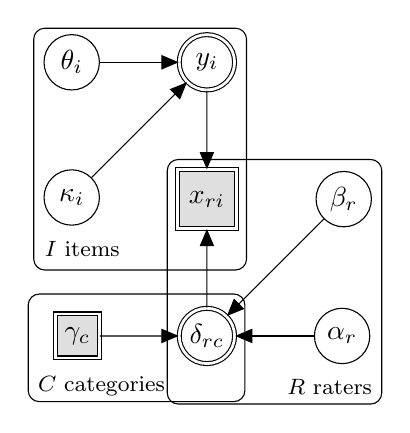
\begin{tikzpicture}[square/.style={regular polygon,regular polygon sides=4}]
%\draw [help lines] (-3,-5) grid (3,5);			

% Define nodes
\node[obsD, double distance=1pt]                        (x) {$x_{\Irater\Iitem}$};
\node[latent, below = of x, double distance = 1pt]      (d) {$\Threshold_{\Irater\Incat}$};
\node[latent, right = of d]                             (a) {$\RaterScale_\Irater$};
\node[latent, right = of x]                             (b) {$\RaterShift_\Irater$};
\node[obsD, left  = of d, double distance = 1pt]        (g) {$\UnBiasedThreshold_\Incat$};

\node[latent, above = of x, double distance = 1pt]      (y) {$\Appraisal_{\Iitem}$};%{$\Appraisal_{\Irater\Iitem}$};
\node[latent, left  = of y]                             (t) {$\ItemTruth_\Iitem$};
%\node[latent, right = of e] 						    (E) {$\zeta_\Irater$};
%\node[latent, right = of tau, draw = none] 				(E) {};
%\node[latent, left  = of e] 						    (tau) {$\ItemDifficulty_\Iitem$};
\node[latent, below  = of t] 						    (tau) {$\ItemDifficulty_\Iitem$};

% Edges
\edge {d}       {x};%
\edge {a, b, g} {d};%
\edge {t, tau}    {y};%
\edge {y}       {x};%
%\edge {E}       {e};%
%\edge {tau}     {e};%

%\plate[text centered] {ni} {(a)(b)(d)(x)(y)}     {$\Trater$ raters };
\plate[text centered] {ni} {(a)(b)(d)(x)}     {$\Trater$ raters };
{\tikzset{plate caption/.append style={below=4pt of #1.south west, xshift = .5cm}}
\plate[text centered, yshift = -.05cm] {ni} {(t)(x)(y)(tau)}            {$\Titem$ items  };
%\plate[text centered, yshift = -.05cm] {ni} {(t)(x)(y)(e)(tau)}            {$\Titem$ items  };
}
{\tikzset{plate caption/.append style={below=4pt of #1.south west, xshift = 0.6cm}}
\plate[text centered, yshift =  .05cm] {nc} {(g)(d)}              {$\Tncat$ categories};
}

\end{tikzpicture}

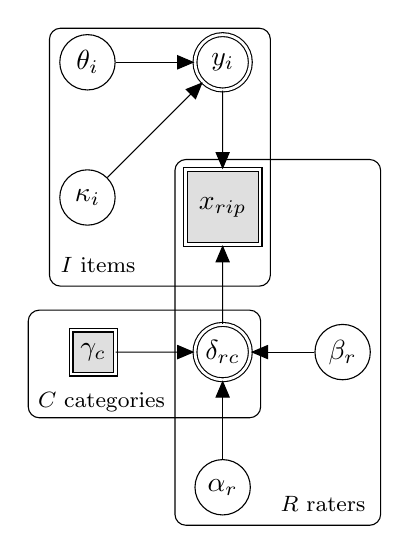
\begin{tikzpicture}[square/.style={regular polygon,regular polygon sides=4}]
%\draw [help lines] (-3,-5) grid (3,5);			

% Define nodes
\node[obsD, double distance=1pt]                         (x) {$x_{\Irater\Iitem\Ipatient}$};
\node[latent, below = of x, double distance = 1pt]      (d) {$\Threshold_{\Irater\Incat}$};
\node[latent, below = of d]                             (a) {$\RaterScale_\Irater$};
\node[latent, right = of d, xshift = -5.5pt]       		(b) {$\RaterShift_\Irater$};
\node[obsD, left  = of d, double distance = 1pt]        (g) {$\UnBiasedThreshold_\Incat$};

\node[latent, above = of x, double distance = 1pt]      (y) {$\Appraisal_{\Iitem}$};%{$\Appraisal_{\Irater\Iitem}$};
%\node[latent, above = of y]                             (e) {$\Error_{\Iitem}$};
\node[latent, left  = of y]                             (t) {$\ItemTruth_\Iitem$};
%\node[latent, right = of e] 						    (E) {$\zeta_\Irater$};
%\node[latent, right = of tau, draw = none] 				(E) {};
%\node[latent, left  = of e] 						    (tau) {$\ItemDifficulty_\Iitem$};
\node[latent, below  = of t] 						    (tau) {$\ItemDifficulty_\Iitem$};

% Edges
\edge {d}       {x};%
\edge {a, b, g} {d};%
\edge {t, tau}    {y};%
\edge {y}       {x};%
%\edge {E}       {e};%
%\edge {tau}     {e};%

%\plate[text centered] {ni} {(a)(b)(d)(x)(y)}     {$\Trater$ raters };
{\tikzset{plate caption/.append style={left=2pt of #1.south east, yshift = .15cm}}
\plate[text centered] {ni} {(a)(b)(d)(x)}     {$\Trater$ raters };
}
{\tikzset{plate caption/.append style={below=4pt of #1.south west, xshift = .5cm}}
	\plate[text centered, yshift = -.05cm] {ni} {(t)(x)(y)(tau)}            {$\Titem$ items  };
	%\plate[text centered, yshift = -.05cm] {ni} {(t)(x)(y)(e)(tau)}            {$\Titem$ items  };
}
{\tikzset{plate caption/.append style={below=4pt of #1.south west, xshift = 0.4cm}}
	\plate[text centered, yshift =  .05cm] {nc} {(g)(d)}              {$\Tncat$ categories};
}

\end{tikzpicture}

%\begin{tikzpicture}[square/.style={regular polygon,regular polygon sides=4}]
%%\draw [help lines] (-3,-5) grid (3,5);
%
%% Define nodes
%\node[obsD, double distance=1pt]                        (x) {$x_{\Irater\Iitem\Ipatient}$};
%\node[latent, below = of x, double distance = 1pt]      (d) {$\Threshold_{\Irater\Incat}$};
%\node[latent, right = of d]                             (a) {$\RaterScale_\Irater$};
%\node[latent, right = of x, xshift = -5.5pt]            (b) {$\RaterShift_\Irater$};
%\node[obsD, left  = of d, double distance = 1pt]        (g) {$\UnBiasedThreshold_\Incat$};
%
%\node[latent, above = of x]                             (y) {$\Appraisal_{\Irater\Iitem\Ipatient}$};
%\node[latent, above = of y]                             (e) {$\Error_{\Irater\Iitem\Ipatient}$};
%\node[latent, left  = of y]                             (t) {$\ItemTruth_{\Iitem\Ipatient}$};
%
%\node[latent, right = of e] 						    (E) {$\zeta_\Irater$};
%\node[latent, left  = of e] 						    (tau) {$\ItemDifficulty_{\Iitem\Ipatient}$};
%
%\node[latent, left  = of t] 						    (l) {$\FactorScore_{\Ipatient\Ilatent}$};
%
%% Edges
%\edge {d}       {x};%
%\edge {a, b, g} {d};%
%\edge {t, e}    {y};%
%\edge {y}       {x};%
%\edge {E}       {e};%
%\edge {tau}     {e};%
%\edge {l}       {t};%
%
%\plate[text centered] {ni} {(a)(b)(d)(x)(y)(e)(E)}     {$\Trater$ raters };
%{\tikzset{plate caption/.append style={below=4pt of #1.south west, xshift = .6cm}}
%	\plate[text centered] {ni} {(t)(x)(y)(e)(tau)}            {$\Titem$ items  };
%}
%{\tikzset{plate caption/.append style={below=4pt of #1.south west, xshift = .4cm}}
%	\plate[text centered] {nc} {(g)(d)}              {$\Tncat$ categories};
%}
%{\tikzset{plate caption/.append style={below=4pt of #1.south west, xshift = .5cm}}
%	\plate[text centered] {ni} {(t)(x)(y)(e)(l)}            {$\Tpatient$ patients  };
%}
%{\tikzset{plate caption/.append style={below=4pt of #1.south west, xshift = .6cm}}
%	\plate[text centered] {ni} {(l)}     {$\Tlatent$ constructs };
%}
%\end{tikzpicture}

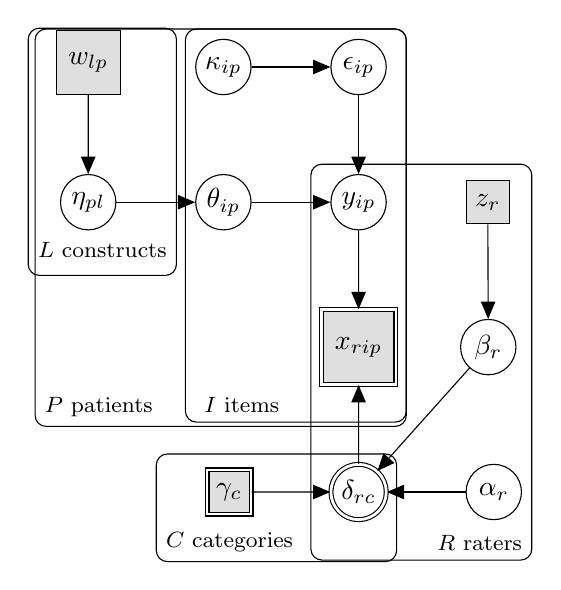
\begin{tikzpicture}[square/.style={regular polygon,regular polygon sides=4}]
%\draw [help lines] (-3,-5) grid (3,5);			

% Define nodes
\node[obsD, double distance=1pt]                         (x) {$x_{\Irater\Iitem\Ipatient}$};
\node[latent, below = of x, double distance = 1pt]      (d) {$\Threshold_{\Irater\Incat}$};
\node[latent, right = of d]                             (a) {$\RaterScale_\Irater$};
\node[latent, right = of x, xshift = -5.5pt]       		(b) {$\RaterShift_\Irater$};
\node[obsD, left  = of d, double distance = 1pt]        (g) {$\UnBiasedThreshold_\Incat$};

\node[latent, above = of x]                             (y) {$\Appraisal_{\Iitem\Ipatient}$};%{$\Appraisal_{\Irater\Iitem\Ipatient}$};
\node[latent, above = of y]                             (e) {$\Error_{\Iitem\Ipatient}$};
\node[latent, left  = of y]                             (t) {$\ItemTruth_{\Iitem\Ipatient}$};

%\node[latent, right = of e] 						    (E) {$\zeta_\Irater$};
\node[latent, right = of e, draw = none] 				(E) {};
\node[latent, left  = of e] 						    (tau) {$\ItemDifficulty_{\Iitem\Ipatient}$};

\node[latent, left  = of t] 						    (l) {$\FactorScore_{\Ipatient\Ilatent}$};

\node[obsD,    right = of y] 						    (z)  {$\RaterCovariate_{\Irater}$};
\node[obsD,   above = of l]  						    (w) {$\PatientCovariate_{\Ilatent\Ipatient}$};


% Edges
\edge {d}       {x};%
\edge {a, b, g} {d};%
\edge {t, e}    {y};%
\edge {z}       {b};%
\edge {y}       {x};%
%\edge {E}       {e};%
\edge {tau}     {e};%
\edge {l}       {t};%
\edge {w}       {l};%

\plate[text centered] {ni} {(a)(b)(d)(x)(y)}     {$\Trater$ raters };
{\tikzset{plate caption/.append style={below=4pt of #1.south west, xshift = .6cm}}
	\plate[text centered] {ni} {(t)(x)(y)(e)(tau)}            {$\Titem$ items  };
}
{\tikzset{plate caption/.append style={below=4pt of #1.south west, xshift = .3cm}}
	\plate[text centered] {nc} {(g)(d)}              {$\Tncat$ categories};
}
{\tikzset{plate caption/.append style={below=4pt of #1.south west, xshift = .5cm}}
	\plate[text centered] {ni} {(t)(x)(y)(e)(l)}            {$\Tpatient$ patients  };
}
{\tikzset{plate caption/.append style={below=4pt of #1.south west, xshift = .6cm,yshift=0cm}}
	\plate[text centered, yshift = -.1cm] {ni} {(l)(w)}     {$\Tlatent$ constructs };
}
\end{tikzpicture}

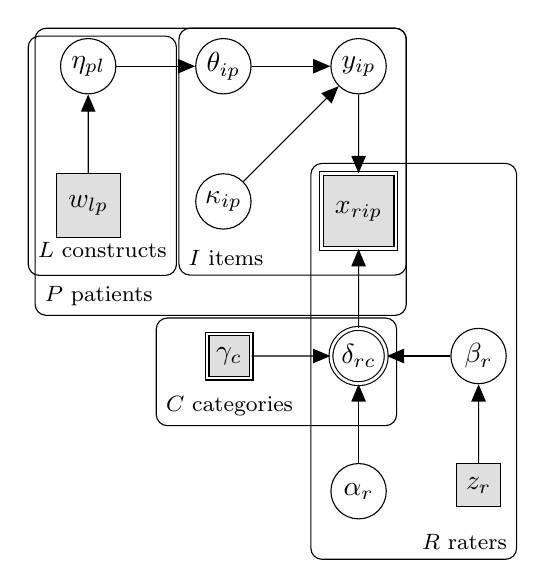
\begin{tikzpicture}[square/.style={regular polygon,regular polygon sides=4}]
%\draw [help lines] (-3,-5) grid (3,5);			

% Define nodes
\node[obsD, double distance=1pt]                         (x) {$x_{\Irater\Iitem\Ipatient}$};
\node[latent, below = of x, double distance = 1pt]      (d) {$\Threshold_{\Irater\Incat}$};
\node[latent, below = of d]                             (a) {$\RaterScale_\Irater$};
\node[latent, right = of d, xshift = -5.5pt]       		(b) {$\RaterShift_\Irater$};
\node[obsD, left  = of d, double distance = 1pt]        (g) {$\UnBiasedThreshold_\Incat$};

\node[latent, above = of x]                             (y) {$\Appraisal_{\Iitem\Ipatient}$};%{$\Appraisal_{\Irater\Iitem\Ipatient}$};
%\node[latent, above = of y]                             (e) {$\Error_{\Iitem\Ipatient}$};
\node[latent, left  = of y]                             (t) {$\ItemTruth_{\Iitem\Ipatient}$};

%\node[latent, right = of e] 						    (E) {$\zeta_\Irater$};
%\node[latent, right = of e, draw = none] 				(E) {};
\node[latent, below  = of t] 						    (tau) {$\ItemDifficulty_{\Iitem\Ipatient}$};

\node[latent, left  = of t] 						    (l) {$\FactorScore_{\Ipatient\Ilatent}$};

\node[obsD,   below = of b] 						    (z)  {$\RaterCovariate_{\Irater}$};
\node[obsD,   below = of l]  						    (w) {$\PatientCovariate_{\Ilatent\Ipatient}$};


% Edges
\edge {d}       {x};%
\edge {a, b, g} {d};%
\edge {t, tau}    {y};%
\edge {z}       {b};%
\edge {y}       {x};%
%\edge {E}       {e};%
%\edge {tau}     {e};%
\edge {l}       {t};%
\edge {w}       {l};%

\plate[text centered] {ni} {(a)(b)(d)(x)(z)}     {$\Trater$ raters };
{\tikzset{plate caption/.append style={below=0pt of #1.south west, xshift = .4cm}}
	\plate[text centered] {ni} {(t)(x)(y)(tau)}            {$\Titem$ items  };
}
{\tikzset{plate caption/.append style={below=4pt of #1.south west, xshift = .3cm}}
	\plate[text centered] {nc} {(g)(d)}              {$\Tncat$ categories};
}
{\tikzset{plate caption/.append style={below=13pt of #1.south west, xshift = .5cm, yshift=0cm}}
	\plate[text centered] {ni} {(t)(x)(y)(l)}            {$\Tpatient$ patients  };
}
{\tikzset{plate caption/.append style={below=4pt of #1.south west, xshift = .6cm,yshift=.1cm}}
	\plate[text centered, yshift = -.1cm] {ni} {(l)(w)}     {$\Tlatent$ constructs };
}
\end{tikzpicture}

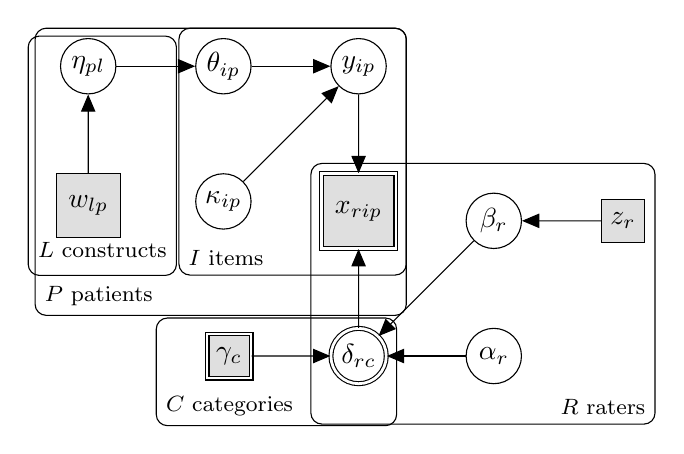
\begin{tikzpicture}[square/.style={regular polygon,regular polygon sides=4}]
%\draw [help lines] (-3,-5) grid (3,5);			

% Define nodes
\node[obsD, double distance=1pt]                         (x) {$x_{\Irater\Iitem\Ipatient}$};
\node[latent, below = of x, double distance = 1pt]      (d) {$\Threshold_{\Irater\Incat}$};
\node[latent, right = of d]                             (a) {$\RaterScale_\Irater$};
\node[latent, above = of a]					       		(b) {$\RaterShift_\Irater$};
\node[obsD, left  = of d, double distance = 1pt]        (g) {$\UnBiasedThreshold_\Incat$};

\node[latent, above = of x]                             (y) {$\Appraisal_{\Iitem\Ipatient}$};%{$\Appraisal_{\Irater\Iitem\Ipatient}$};
%\node[latent, above = of y]                             (e) {$\Error_{\Iitem\Ipatient}$};
\node[latent, left  = of y]                             (t) {$\ItemTruth_{\Iitem\Ipatient}$};

%\node[latent, right = of e] 						    (E) {$\zeta_\Irater$};
%\node[latent, right = of e, draw = none] 				(E) {};
\node[latent, below  = of t] 						    (tau) {$\ItemDifficulty_{\Iitem\Ipatient}$};

\node[latent, left  = of t] 						    (l) {$\FactorScore_{\Ipatient\Ilatent}$};

\node[obsD,   right = of b] 						    (z)  {$\RaterCovariate_{\Irater}$};
\node[obsD,   below = of l]  						    (w) {$\PatientCovariate_{\Ilatent\Ipatient}$};


% Edges
\edge {d}       {x};%
\edge {a, b, g} {d};%
\edge {t, tau}    {y};%
\edge {z}       {b};%
\edge {y}       {x};%
%\edge {E}       {e};%
%\edge {tau}     {e};%
\edge {l}       {t};%
\edge {w}       {l};%

\plate[text centered] {ni} {(a)(b)(d)(x)(z)}     {$\Trater$ raters };
{\tikzset{plate caption/.append style={below=0pt of #1.south west, xshift = .4cm}}
	\plate[text centered] {ni} {(t)(x)(y)(tau)}            {$\Titem$ items  };
}
{\tikzset{plate caption/.append style={below=4pt of #1.south west, xshift = .3cm}}
	\plate[text centered] {nc} {(g)(d)}              {$\Tncat$ categories};
}
{\tikzset{plate caption/.append style={below=13pt of #1.south west, xshift = .5cm, yshift=0cm}}
	\plate[text centered] {ni} {(t)(x)(y)(l)}            {$\Tpatient$ patients  };
}
{\tikzset{plate caption/.append style={below=4pt of #1.south west, xshift = .6cm,yshift=.1cm}}
	\plate[text centered, yshift = -.1cm] {ni} {(l)(w)}     {$\Tlatent$ constructs };
}
\end{tikzpicture}


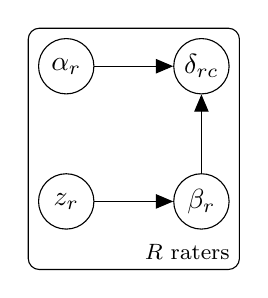
\begin{tikzpicture}[square/.style={regular polygon,regular polygon sides=4}]
%\draw [help lines] (-3,-5) grid (3,5);			

\node[latent]      			(d) {$\Threshold_{\Irater\Incat}$};
\node[latent, left  = of d] (a) {$\RaterScale_\Irater$};
\node[latent, below = of d] (b) {$\RaterShift_\Irater$};
\node[latent, left  = of b] (z) {$z_\Irater$};

% Edges
\edge {a, b} {d}%
\edge {z}    {b}%

\plate[text centered] {ni} {(a)(b)(d)(z)}     {$\Trater$ raters };

\end{tikzpicture}



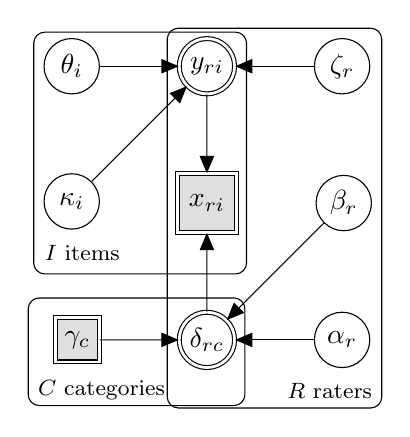
\begin{tikzpicture}[square/.style={regular polygon,regular polygon sides=4}]
%\draw [help lines] (-3,-5) grid (3,5);			

% Define nodes
\node[obsD, double distance=1pt]                        (x) {$x_{\Irater\Iitem}$};
\node[latent, below = of x, double distance = 1pt]      (d) {$\Threshold_{\Irater\Incat}$};
\node[latent, right = of d]                             (a) {$\RaterScale_\Irater$};
\node[latent, right = of x]                             (b) {$\RaterShift_\Irater$};
\node[obsD, left  = of d, double distance = 1pt]        (g) {$\UnBiasedThreshold_\Incat$};

\node[latent, above = of x, double distance = 1pt]      (y) {$\Appraisal_{\Irater\Iitem}$};
\node[latent, left  = of y]                             (t) {$\ItemTruth_\Iitem$};
\node[latent, right = of y] 						    (z) {$\zeta_\Irater$};
\node[latent, below  = of t] 						    (tau) {$\ItemDifficulty_\Iitem$};

% Edges
\edge {d}       {x};%
\edge {a, b, g} {d};%
\edge {t, tau,z}    {y};%
\edge {y}       {x};%
%\edge {E}       {e};%
%\edge {tau}     {e};%

%\plate[text centered] {ni} {(a)(b)(d)(x)(y)}     {$\Trater$ raters };
\plate[text centered] {ni} {(a)(b)(d)(x)(y)(z)}     {$\Trater$ raters };
{\tikzset{plate caption/.append style={below=4pt of #1.south west, xshift = .5cm}}
	\plate[text centered, yshift = -.05cm] {ni} {(t)(x)(y)(tau)}            {$\Titem$ items  };
	%\plate[text centered, yshift = -.05cm] {ni} {(t)(x)(y)(e)(tau)}            {$\Titem$ items  };
}
{\tikzset{plate caption/.append style={below=4pt of #1.south west, xshift = 0.6cm}}
	\plate[text centered, yshift =  .05cm] {nc} {(g)(d)}              {$\Tncat$ categories};
}
\end{tikzpicture}

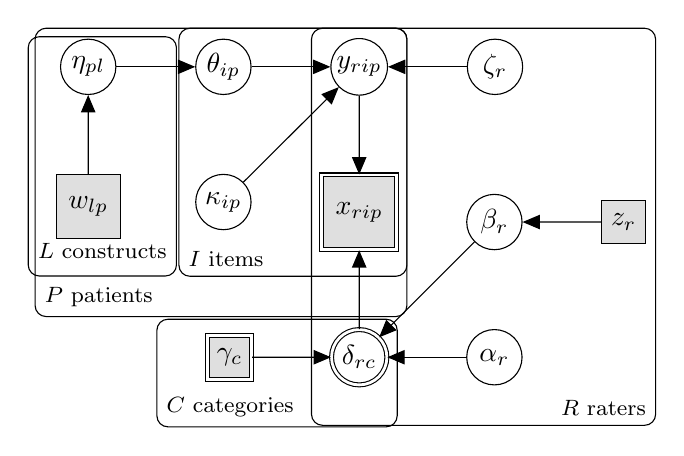
\begin{tikzpicture}[square/.style={regular polygon,regular polygon sides=4}]
%\draw [help lines] (-3,-5) grid (3,5);			

% Define nodes
\node[obsD, double distance=1pt]                         (x) {$x_{\Irater\Iitem\Ipatient}$};
\node[latent, below = of x, double distance = 1pt]      (d) {$\Threshold_{\Irater\Incat}$};
\node[latent, right = of d]                             (a) {$\RaterScale_\Irater$};
\node[latent, above = of a]					       		(b) {$\RaterShift_\Irater$};
\node[obsD, left  = of d, double distance = 1pt]        (g) {$\UnBiasedThreshold_\Incat$};

\node[latent, above = of x]                             (y) {$\Appraisal_{\Irater\Iitem\Ipatient}$};
\node[latent, left  = of y]                             (t) {$\ItemTruth_{\Iitem\Ipatient}$};

\node[latent, right = of y] 						    (zeta) {$\zeta_\Irater$};
\node[latent, below  = of t] 						    (tau) {$\ItemDifficulty_{\Iitem\Ipatient}$};

\node[latent, left  = of t] 						    (l) {$\FactorScore_{\Ipatient\Ilatent}$};

\node[obsD,   right = of b] 						    (z)  {$\RaterCovariate_{\Irater}$};
\node[obsD,   below = of l]  						    (w) {$\PatientCovariate_{\Ilatent\Ipatient}$};


% Edges
\edge {d}       {x};%
\edge {a, b, g} {d};%
\edge {t,zeta, tau}    {y};%
\edge {z}       {b};%
\edge {y}       {x};%
%\edge {E}       {e};%
%\edge {tau}     {e};%
\edge {l}       {t};%
\edge {w}       {l};%

\plate[text centered] {ni} {(a)(b)(d)(x)(z)(y)(zeta)}     {$\Trater$ raters };
{\tikzset{plate caption/.append style={below=0pt of #1.south west, xshift = .4cm}}
	\plate[text centered] {ni} {(t)(x)(y)(tau)}            {$\Titem$ items  };
}
{\tikzset{plate caption/.append style={below=4pt of #1.south west, xshift = .3cm}}
	\plate[text centered] {nc} {(g)(d)}              {$\Tncat$ categories};
}
{\tikzset{plate caption/.append style={below=13pt of #1.south west, xshift = .5cm, yshift=0cm}}
	\plate[text centered] {ni} {(t)(x)(y)(l)}            {$\Tpatient$ patients  };
}
{\tikzset{plate caption/.append style={below=4pt of #1.south west, xshift = .6cm,yshift=.1cm}}
	\plate[text centered, yshift = -.1cm] {ni} {(l)(w)}     {$\Tlatent$ constructs };
}
\end{tikzpicture}

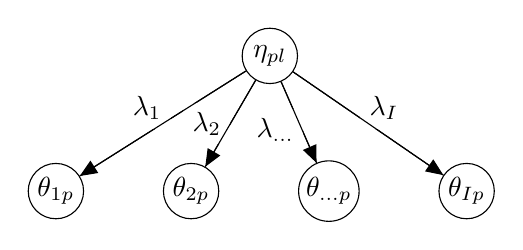
\begin{tikzpicture}[square/.style={regular polygon,regular polygon sides=4}]
%\draw [help lines] (-3,-5) grid (3,5);			

\node[latent]                              (t1)  {$\ItemTruth_{1\Ipatient}$};
\node[latent, right = of t1]               (t2)  {$\ItemTruth_{2\Ipatient}$};
\node[latent, right = of t2]               (t3)  {$\ItemTruth_{\dots\Ipatient}$};
\node[latent, right = of t3]               (t4)  {$\ItemTruth_{\Titem\Ipatient}$};
\node[latent, above = of t2, xshift = 1cm] (eta) {$\FactorScore_{\Ipatient\Ilatent}$};

\draw (eta) -- (t1) node [midway, fill=white, xshift = -.2cm, 	yshift = .2cm]  {$\FactorRegression_{1}$};
\draw (eta) -- (t2) node [midway, fill=white, xshift = -.3cm, 	yshift = 0cm]   {$\FactorRegression_{2}$};
\draw (eta) -- (t3) node [midway, fill=white, xshift = -.3cm, 	yshift = -.1cm]	{$\FactorRegression_{\dots}$};
\draw (eta) -- (t4) node [midway, fill=white, xshift = .2cm,	yshift = .2cm]  {$\FactorRegression_{\Titem}$};

% Edges
\edge {eta} {t1, t2, t3, t4}%
\end{tikzpicture}

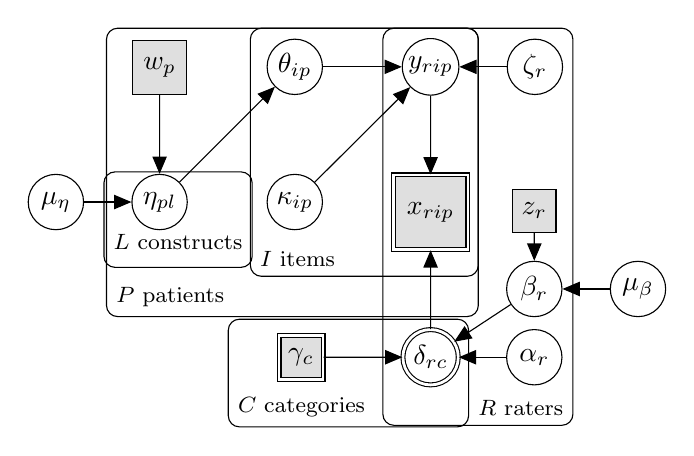
\begin{tikzpicture}[square/.style={regular polygon,regular polygon sides=4}]
%\draw [help lines] (-3,-5) grid (3,5);			

% Define nodes
\node[obsD, double distance=1pt]                        (x) 	{$x_{\Irater\Iitem\Ipatient}$};
\node[latent, below = of x, double distance = 1pt]      (d) 	{$\Threshold_{\Irater\Incat}$};
\node[latent, right = of d, xshift = -.4cm]                             (a) 	{$\RaterScale_\Irater$};
\node[latent, above = of a, yshift=-.85cm]				(b) 	{$\RaterShift_\Irater$};
\node[obsD, left  = of d, double distance = 1pt]        (g) 	{$\UnBiasedThreshold_\Incat$};

\node[latent, above = of x]                             (y)		{$\Appraisal_{\Irater\Iitem\Ipatient}$};
\node[latent, left  = of y]                             (t)		{$\ItemTruth_{\Iitem\Ipatient}$};

\node[latent, right = of y, xshift = -.4cm]			    (zeta) 	{$\zeta_\Irater$};
\node[latent, below  = of t] 						    (tau) 	{$\ItemDifficulty_{\Iitem\Ipatient}$};

\node[latent, left  = of tau] 						    (l) 	{$\FactorScore_{\Ipatient\Ilatent}$};

%\node[obsD,   above = of b, yshift = +.65cm]		    (z)  	{$\RaterCovariate_{\Irater}$};
\node[obsD,   above = of b, yshift = -.65cm]		    (z)  	{$\RaterCovariate_{\Irater}$};
\node[obsD,   above = of l]  						    (w)		{$\PatientCovariate_{\Ipatient}$};
\node[latent, right = of b, xshift = -.4cm]			    (muz)  	{$\mu_{\RaterShift}$};
\node[latent, left  = of l, xshift = +.4cm]			    (mueta)	{$\mu_{\FactorScore}$};


% Edges
\edge {d}       	{x};%
\edge {a, b, g}		{d};%
\edge {t,zeta, tau} {y};%
\edge {z, muz}      {b};%
\edge {y}       	{x};%
\edge {l}      		{t};%
\edge {w, mueta}	{l};%

\plate[text centered] {ni} {(a)(b)(d)(x)(z)(y)(zeta)}     {$\Trater$ raters };
{\tikzset{plate caption/.append style={below=0pt of #1.south west, xshift = .4cm}}
	\plate[text centered] {ni} {(t)(x)(y)(tau)}            {$\Titem$ items  };
}
{\tikzset{plate caption/.append style={below=4pt of #1.south west, xshift = .3cm}}
	\plate[text centered] {nc} {(g)(d)}              {$\Tncat$ categories};
}
{\tikzset{plate caption/.append style={below=13pt of #1.south west, xshift = .5cm, yshift=0cm}}
	\plate[text centered] {ni} {(t)(x)(y)(l)}            {$\Tpatient$ patients  };
}
{\tikzset{plate caption/.append style={below=4pt of #1.south west, xshift = .6cm,yshift=.1cm}}
	\plate[text centered, yshift = -.1cm] {ni} {(l)}     {$\Tlatent$ constructs };
}

%\plate[text centered] {nzp} {(mueta)}	{$\Tncat$ categories};
%\plate[text centered] {nzr} {(muz)}		{$\Tncat$ categories};
\end{tikzpicture}

\end{document}


